\documentclass{article}

\usepackage{eaj}
\usepackage{geometry}
\geometry{
    a4paper
}

\title{\vspace{-2cm} \textbf{Labyrintmanus}\\[.4em] \large TPD4114 Visuell formidling \\[1em] Erik André Jakobsen \\[.4em] Fredag 29. november \vspace{-1.5cm}}
\date{}
\author

\definecolor{primary}{HTML}{FF8000}
\definecolor{primary-dark}{HTML}{A30000}
\definecolor{secondary}{HTML}{00AFB5}
\definecolor{secondary-dark}{HTML}{004777}
\definecolor{highlight}{HTML}{EFD28D}

\newcommand{\hl}[2][primary-dark]{\textcolor{#1}{#2}}

\begin{document}
\maketitle

\section*{Informasjon}
\begin{center}
    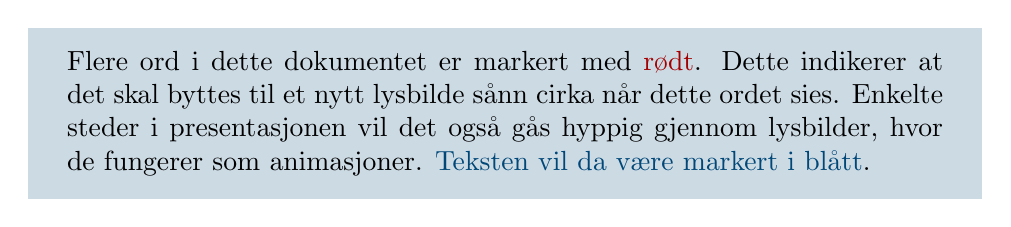
\begin{tikzpicture}
        \node [fill=secondary-dark!20, text width=\linewidth-1cm, align=justify, inner xsep=5mm, inner ysep=3mm] at (0, 0)
            {Flere ord i dette dokumentet er \mbox{markert} med \hl{rødt}. Dette \mbox{indikerer} at det skal byttes til et nytt lysbilde sånn cirka når dette ordet sies. Enkelte steder i presentasjonen vil det også gås hyppig gjennom lysbilder, hvor de fungerer som animasjoner. \hl[secondary-dark]{Teksten vil da være markert i blått}.};
    \end{tikzpicture}
\end{center}

\begin{center}
    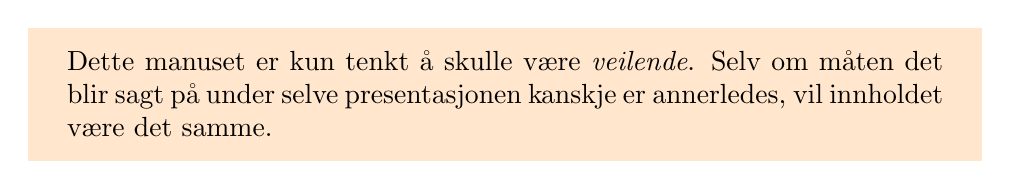
\begin{tikzpicture}
        \node [fill=primary!20, text width=\linewidth-1cm, align=justify, inner xsep=5mm, inner ysep=3mm] at (0, 0)
            {Dette manuset er kun tenkt å skulle være \emph{veilende}. Selv om måten det blir sagt på under selve presentasjonen kanskje er annerledes, vil innholdet være det samme.};
    \end{tikzpicture}
\end{center}

\section*{Presentasjonen}
Dette er en labyrint. Vi starter på toppen, og målet er å finne veien til bunnen. Denne er rimelig \hl{lett}. \hl{Her} er en litt større en, som det hadde tatt en stund å \hl{løse}. \hl{Denne} labyrinten er bortimot umulig å \hl{løse}. For å få det til måtte jeg bruke en datamsaskin. Men før jeg kunne gjøre det, måtte jeg oversette den til et språk datamaskinen forstår -- \hl{nullere} og enere.

\hl{Som} alle andre bilder på en skjerm er dette bilde sammensatt av \hl{piksler}: mange små punkter. Akkurat denne labyrinten består av 100 piksler. \hl{Vi} tilegner de svarte pikslene verdien \texttt{0}, og de hvite pikslene verdien \texttt{1}. Det betyr at der vi ser en labyrint, ser datamaskinen \hl{dette}. Det blir litt vanskelig for oss å følge med med bare tall, så vi \hl{beholder} labyrinten under.

Det neste vi må gjøre er å lære datamaskinen reglene. Vi ønsker å komme oss fra \hl{hit} til \hl{hit}, og vi har kun lov å gå rett opp og ned eller til siden. Den enkleste måten å finne løsningen på er å ta et vilkårlig lovlig steg, og sjekke om vi er kommet frem. Vi må hele tiden lagre hvor vi tar steget fra, slik at når vi til slutt kommer frem, så kan vi følge stegene våre tilbake til utgangspunktet. Vi vil altså begynne med å \hl{ta} et steg, og sjekke om det var hit vi skulle. Det var det ikke, så vi \hl{tar} et steg til, sjekker igjen, vi er fremdeles ikke fremme, \hl{nytt} steg. \hl[secondary-dark]{Dette fortsetter videre, steg for steg, sjekk for sjekk, og det kan ta en} \hl{stund}. \hl{Endelig} er vi til slutt fremme. Vi tar et \hl{steg}, sjekker om vi er fremme -- og det er vi! \hl[secondary-dark]{Da er det bare å se hvor vi kom fra, og gå tilbake til start, steg for steg.} Dermed har vi \hl{løsningen}!

\hl{Men}.

Dette er ikke så veldig \hl{effektivt}, og, kanskje verre, om det finnes flere løsninger er det ingen garanti for at vi finner den \hl{korteste}.

En av grunnene til at dette tar en stund er at vi foretar flere valg enn vi trenger. Dersom det er en \hl{korridor} i labyrinten vår, er det ingen grunn til å gå steg for steg og sjekke underveis. Vi vet jo at vi må gå hele veien, så hvorfor ikke bare \hl{erstatte} korridoren med et eneste langt steg? Dersom det skulle være mulig å \hl{svinge} underveis, kan vi bare legge inn et \hl{veikryss}. Om det er \hl{behov} for det, kan vi selvfølgelig gi \hl{muligheten} for å gå i alle fire lovlige retninger i et kryss.

Fremgangsmåten vår blir da litt \hl{annerledes}. Etter å ha markert start og stopp, \hl{setter} vi \hl{inn} veikryss i disse rutene. Deretter går vi gjennom hele labyrinten, rute for rute, og ser om det burde være et veikryss der. Vi \hl{starter} med et hjørne: Her må vi nesten svinge, så vi setter inn et \hl{kryss}. I den \hl{neste} ruten har vi ikke noe annet valg enn å gå til høyre og til venstre, så da går vi bare videre. \hl{Da} kommer vi til et veikryss, så vi setter det inn. Nå må vi også begynne å \hl{koble} \hl{kryssene} vi kan nå fra denne ruten sammen. \hl[secondary-dark]{Slik fortsetter vi: Rute for rute ser vi om det burde være et veikryss der. Hvis ja, sett det inn, og koble det sammen med de andre kryssene}. Dette tar naturligvis også en \hl{stund}, men til slutt har vi laget et helt \hl{nettverk}. Nå \hl{trenger} vi egentlig ikke labyrinten lenger, problemet vårt nå er å løse nettverket.

Før vi begynner med det, gjør vi en ny observasjon: Det finnes en del kryss som ikke gjør noe annet enn å skifte retning, det er ikke noe valg å ta der. Det betyr at vi ikke trenger dem, og vi \hl{fjerner} dem.

Deretter må vi ha et mål på hvor lang hver strekning er, siden vi vil finne den korteste veien. Jeg har gjort det enkelt og bare \hl{telt} piksler, endepunktene inkludert. Mellom start og første veikryss er dermed avstanden to, siden den veien strekker seg over to piksler. Vi kan gjerne kalle det meter. For å få det til å se litt bedre ut tar jeg og \hl{strekker} ut noen av veien, men det er utelukkende visuelt for denne presentasjonen, og har ingenting å si for valg av vei.

Deretter er det bare å \hl{starte}. Etterhvert som vi kommer frem vil hvert veikryss få et tall som indikerer hvor langt det er å komme seg dit fra start. Som før tar vi også vare på hvor vi kommer fra, slik at vi kan finne veien tilbake.

Først har vi ikke så mye valg: Vi må nesten gå \hl{ned}, og vi må gå to meter for å komme dit. Herfra kan vi velge: Vi kan gå til \hl{venstre}, og komme hit. Da har vi totalt gått \hl{syv} meter. To meter fra start til det første krysset, og så fem meter videre derfra igjen. Vi kan også velge å gå til \hl{høyre} og komme hit, med en total distanse på \hl{seks} meter.

Siden vi ønsker å finne kortest mulig vei, velger vi å alltid sjekke mulighetene fra veikrysset som er \emph{nærmest start}. Det er nå veikrysset som er 6 meter unna, så vi ser på mulighetene derfra. Vi kan komme oss ned \hl{hit} ved å gå \hl{tolv} meter, eller \hl{hit} ved å gå \hl{fjorten} meter.

Det nærmeste veikrysset nå er dette til venstre, så vi ser på mulighetene derfra. Vi kan komme oss \hl{hit} ved å gå \hl{tolv} meter. Det andre alternativet er å gå \hl{denne} veien, men siden begge er like lange blir det fremdeles tolv meter.

Nå som vi har to veikryss som begge er like langt unna har det ikke noe å si hvilket vi velger først. Vi velger det til høyre, og ser på \hl{denne} veien. Da kan vi komme oss hit, men ved å gå denne veien ville det ta femten meter, og vi klarer det allerede på tolv. Derfor endrer vi ikke veikryssets avstand.

\hl[secondary-dark]{Vi fortsetter på denne måten: Velger krysset som er nærmest, ser hvor vi kan komme oss og hvor langt det er dit, og gjentar deretter prosessen}, helt til vi kommer i \hl{mål}! Vi slutter derimot ikke nå, siden for alt vi vet, kan det hende at det finnes en bedre vei ... kanskje en snarvei herfra, for eksempel? \hl[secondary-dark]{Derfor fortsetter vi å sjekke}, helt til \emph{målet er det nærmeste krysset}. Da vet vi at vi har funnet den korteste veien, og som \hl{før} så \hl[secondary-dark]{går vi steg for steg tilbake til utgangspunktet}. Da har vi funnet \hl{løsningen} på labyrinten!

Dette er \hl{garantert} den korteste veien, men ikke bare det -- avstanden vi noterte oss for veikryssene underveis er den korteste mulige avstanden til \hl{alle} veikryssene!

Alt dette er vel og bra, men ... \hl{hvem} bryr seg?

Vel, noen som bryr seg er \hl{de} folkene her. Labyrintene det dreier seg om kan være \hl{tognettverk}, \hl{vennenettverk}, eller kart hvor målet er å finne beste \hl{veibeskrivelse} eller beste rute for en \hl{taxi} i nærheten.

Det var det jeg hadde. \hl{Tusen} takk for meg!
\end{document}